It was initially found that the stoachastic nature of the simulation caused it
to be very hard to evaluate and increases in the shark's fitness value did not have any
major impact. This stochastic behaviour can be seen in figure
\ref{fig:walnutfitness}, where the simulation was run using a random behaviour
in the shark instead of the neural network.\\
\\
When applying the neural betwork it was seen that a highly stochastic
behaviour remained in the model, which in turn meant that the maximum fitness
value seen in figure \ref{sub@fig:aifitness1} means very little for the
success of the shark when applying this weight matrix to a simulation run.\\
\\
\begin{figure}[htp]
\begin{center}
\begin{subfigure}[b]{0.5\textwidth}
 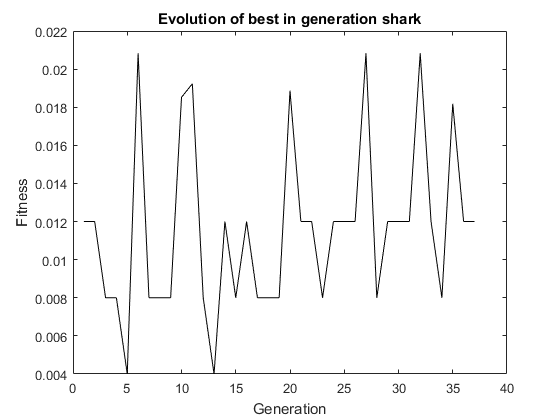
\includegraphics[width=\textwidth]{figs/walnut.png}
 \caption[]{Random behaviour.}
 \label{fig:walnutfitness}
\end{subfigure}~
\begin{subfigure}[b]{0.5\textwidth}
 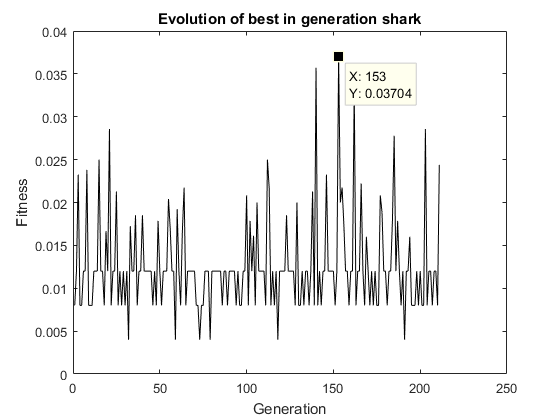
\includegraphics[width=\textwidth]{figs/aifitness1.png}
 \caption[]{Neural network.}
 \label{fig:aifitness1}
\end{subfigure}
\caption{Fitness curves for the shark.}
\label{fig:fitness1}
\end{center}
\end{figure}

By tweaking the creep rate of the GA it was possible to reduce the
stochasiticity caused by the optmization to an acceptable amount, and when the
neural network was applied to these settings it was seen that the shark made
progress in finding a good hunting strategy, as seen in figure
\ref{fig:aifitness2}.
When the best performing weight matrix was simulated visually it was
determined that the shark had evolved towards finding a good hunting strategy.\\
\\
\begin{figure}[htp]
\begin{center}
  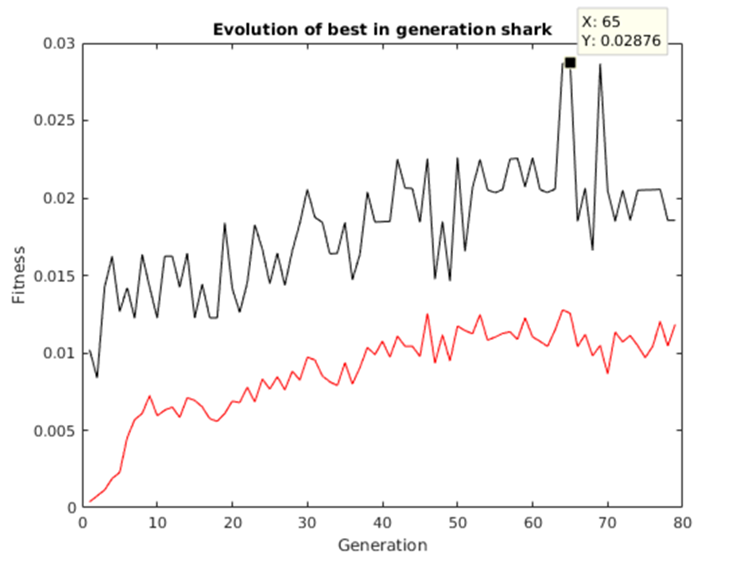
\includegraphics[width=\textwidth]{figs/goodfit.png}
  \caption[]{Shark fitness history after parameter tweaking with neural
  network.}
  \label{fig:aifitness2}
\end{center}
\end{figure}

Due to the vast amount of parameters in this model it was found to be of
interest to document which parameters had the most impact on the result. The
parameters that were found to have the greatest impact are presented in table
\ref{tab:params}. Due to the dependent nature of fish speed, shark
speed and shark view distance these will be presented in text instead of the
table.\\
\\
``Fish speed'' and ``Shark speed'' have a direct relationship to
eachother in that if the fish have a greater speed than the shark they will
never get caught. This is further supported by analyzing real world
prey-predator relationship, where time and again predators are faster than
prey. The speed needs to be set at the right amount as too much speed may cause
the shark to over-shoot the fish shoal, whilst to low speed may cause its
stamina to drain before ever even reaching the shoal.\\
\\
The ``Shark view
distance'' needs to be set at a large enough amount for the shark not to lose
sight of the fish, at least not for any longer period of time, but it can not
be set too big as the shark may become all-seeing and break the aim to keep
close to the biological limits of sharks.\\
\\
``Shark stamina" is increased to
increase the evaluation time for the shark in order to lessen the effects of
initial conditions ``luck" that may affect the shark.\\
\\
\begin{table}[h]
\begin{tabular}{|c|c|c|c|}
\hline
\textbf{Parameter} & \textbf{Change} & \textbf{Effect} & \textbf{Consequence}\\
\hline
Creep rate & Decrease & Less stochasticity & Smaller search space \\
\hline
Hidden layers & $1\rightarrow3$ & Better fitness &  Heavier computation\\
\hline
\hline
Fish speed & Increase & See text & Can't $>$Shark speed \\
\hline
Shark speed & Increase & See text & Can't $<$Fish speed \\
\hline
\hline
Shark stamina & Increase & Decrease ``luck'' & Longer evaluations
\\
\hline
Shark view distance & Increase & See text & Too much=All-seeing \\
\hline
\end{tabular}
\caption{Parameter values and their associated effect.}
\label{tab:params}
\end{table}

When compared to a ``classical'' AI that does not use neural networking, it was
shown that the fitness value of this programmed shark remained relatively
constant, while the neural network shark varies between vastly outperforming it
and giving a slightly lower fitness value.
